
%(BEGIN_QUESTION)
% Copyright 2006, Tony R. Kuphaldt, released under the Creative Commons Attribution License (v 1.0)
% This means you may do almost anything with this work of mine, so long as you give me proper credit

How much pressure, in units of ``inches of water column,'' is being applied to the right-hand tube of this U-tube water manometer?

$$\includegraphics[width=15.5cm]{i00163x01.eps}$$

Also, convert this pressure into units of Pascals.

\vskip 20pt \vbox{\hrule \hbox{\strut \vrule{} {\bf Suggestions for Socratic discussion} \vrule} \hrule}

\begin{itemize}
\item{} How much {\it differential pressure} is registered by this manometer?
\end{itemize}

\underbar{file i00163}
%(END_QUESTION)





%(BEGIN_ANSWER)

Pressure applied to right-hand tube = 26.5 "W.C = 6600.8 Pa.

\vskip 10pt

Follow-up question: demonstrate how we could have arrived at an approximate answer by using rounded figures for our unit-conversion constants, and ``mental math'' instead of a calculator.

%(END_ANSWER)





%(BEGIN_NOTES)

The total distance between the two water columns is 6.5 inches (3.25 inches + 3.25 inches = 6.5 inches).  Since manometers are essentially differential pressure instruments, the two pressures must {\it differ} by 6.5 inches of water column.

Since the right-hand water column is being ``pushed down'' more than the left-hand column, we know the pressure on the right is greater than the pressure on the left.  Given a differential pressure of 6.5 "W.C., and a left-hand applied pressure of 20 "W.C., the right-hand pressure must be the sum, or 26.5 "W.C.

%INDEX% Measurement, pressure: manometer

%(END_NOTES)


